\chapter{Leçon 26: D'Tessy an de Louis}

Dës Lektioun beschäftegt sech mat der Liewensgeschicht (Biografie) vun der Tessy Antony-de Nassau an dem Prënz Louis vu Lëtzebuerg. Mir léieren iwwer hir Familljen, wéi si sech kenne geléiert hunn an hire Liewenswee. Mir studéieren och d'Konjugatioun vum Verb \textbf{heeschen} an de Gebrauch vum Verb \textbf{sech verloben}, an e puer typesch lëtzebuergesch Ausdréck. \textit{Cette leçon traite de la biographie de Tessy Antony-de Nassau et du prince Louis de Luxembourg. Nous apprenons à connaître leurs familles, comment ils se sont rencontrés et leur parcours de vie. Nous étudions également la conjugaison du verbe \textbf{heeschen} (mendier) et l'utilisation du verbe \textbf{sech verloben} (se fiancer), ainsi que quelques expressions typiques luxembourgeoises. / This lesson deals with the biography of Tessy Antony-de Nassau and Prince Louis of Luxembourg. We learn about their families, how they met, and their life paths. We also study the conjugation of the verb \textbf{heeschen} (to beg) and the use of the verb \textbf{sech verloben} (to get engaged), and some typical Luxembourgish expressions.}

\vspace{1em}

\section[D'Geschicht vun der Tessy an dem Louis / L'histoire de Tessy et Louis / The story of Tessy and Louis]{D'Geschicht vun der Tessy an dem Louis \\/ L'histoire de Tessy et Louis \\/ The story of Tessy and Louis}

Hei ass eng kuerz Biographie iwwer d'Tessy Antony-de Nassau an de Prënz Louis vu Lëtzebuerg, déi eis hëlleft de Sproochgebrauch ze üben: \\
\textit{Voici une courte biographie sur Tessy Antony-de Nassau et le prince Louis de Luxembourg, qui nous aide à pratiquer l'usage de la langue : / Here is a short biography about Tessy Antony-de Nassau and Prince Louis of Luxembourg, which helps us practice language usage:}

\vspace{1em}

\noindent\textbf{1. Tessy Antony ass d'Duechter vum François Antony, deen en Daachdecker war, a vun der Régine Antony, déi eng Hausfrau war. De Louis ass de Jong vum Groussherzog Henri a vun der Groussherzogin Maria Teresa.}\\
\textit{Tessy Antony} (Tessy Antony) \textit{ass d'Duechter} (est la fille / is the daughter) \textit{vum François Antony, deen en Daachdecker war} (de François Antony, qui était couvreur / of François Antony, who was a roofer), \textit{a vun der Régine Antony, déi eng Hausfrau war} (et de Régine Antony, qui était femme au foyer / and of Régine Antony, who was a homemaker). \textit{De Louis} (Louis) \textit{ass de Jong} (est le fils / is the son) \textit{vum Groussherzog Henri} (du Grand-Duc Henri / of Grand Duke Henri) \textit{a vun der Groussherzogin Maria Teresa} (et de la Grande-Duchesse Maria Teresa / and of Grand Duchess Maria Teresa).\\
$\rightarrow$ Français : \textit{Tessy Antony est la fille de François Antony, qui était couvreur, et de Régine Antony, qui était femme au foyer. Louis est le fils du Grand-Duc Henri et de la Grande-Duchesse Maria Teresa.}\\
$\rightarrow$ English : \textit{Tessy Antony is the daughter of François Antony, who was a roofer, and of Régine Antony, who was a homemaker. Louis is the son of Grand Duke Henri and Grand Duchess Maria Teresa.}\\[0.5em]

\noindent\textbf{2. Si hu sech zu Lëtzebuerg kenne geléiert, nodeems d'Tessy aus dem Kosovo zréckkomm war. De Prënz Louis huet säi Führerschäin an der Arméi gemaach, an d'Tessy huet seng Aen an engem Aentest kontrolléiert. Et war Léift op den éischte Bléck!}\\
\textit{Si hu sech... kenne geléiert} (Ils se sont rencontrés / They met) \textit{zu Lëtzebuerg} (au Luxembourg / in Luxembourg), \textit{nodeems d'Tessy} (après que Tessy / after Tessy) \textit{aus dem Kosovo zréckkomm war} (était revenue du Kosovo / had returned from Kosovo). \textit{De Prënz Louis} (Le prince Louis / Prince Louis) \textit{huet säi Führerschäin... gemaach} (a passé son permis de conduire / got his driving license) \textit{an der Arméi} (à l'armée / in the army), \textit{an d'Tessy huet seng Aen... kontrolléiert} (et Tessy a contrôlé ses yeux / and Tessy checked his eyes) \textit{an engem Aentest} (dans un test visuel / in an eye test). \textit{Et war Léift} (C'était l'amour / It was love) \textit{op den éischte Bléck} (au premier regard / at first sight).\\
$\rightarrow$ Français : \textit{Ils se sont rencontrés au Luxembourg, après le retour de Tessy du Kosovo. Le prince Louis passait son permis de conduire à l'armée, et c'est Tessy qui a contrôlé sa vue lors d'un test oculaire. Ce fut le coup de foudre !}\\
$\rightarrow$ English : \textit{They met in Luxembourg, after Tessy had returned from Kosovo. Prince Louis was getting his driving license in the army, and Tessy checked his eyesight in an eye test. It was love at first sight!}\\[0.5em]

\noindent\textbf{3. D'Koppel huet sech am Joer 2006 zu Gilsdref verloobt a bestuet, nodeems hiren éischte Jong, de Gabriel, op d'Welt komm war.}\\
\textit{D'Koppel} (Le couple / The couple) \textit{huet sech... verloobt a bestuet} (s'est fiancé et marié / got engaged and married) \textit{am Joer 2006} (en l'an 2006 / in the year 2006) \textit{zu Gilsdref} (à Gilsdorf / in Gilsdorf), \textit{nodeems hiren éischte Jong} (après que leur premier fils / after their first son), \textit{de Gabriel} (Gabriel), \textit{op d'Welt komm war} (était venu au monde / had come into the world).\\
$\rightarrow$ Français : \textit{Le couple s'est fiancé et marié en 2006 à Gilsdorf, après la naissance de leur premier fils, Gabriel.}\\
$\rightarrow$ English : \textit{The couple got engaged and married in 2006 in Gilsdorf, after their first son, Gabriel, was born.}\\[0.5em]

\noindent\textbf{4. Well de Prënz Louis ouni d'Zoustëmmung vum Haff bestuet ass, huet hien op seng Trounrechter a fir seng Kanner verzicht. Am Joer 2007 krute si hiren zweete Jong Noah, an am Joer 2009 gouf d'Tessy vum Groussherzog zur Prinzessin ernannt.}\\
\textit{Well de Prënz Louis... bestuet ass} (Parce que le prince Louis s'est marié / Because Prince Louis married) \textit{ouni d'Zoustëmmung vum Haff} (sans le consentement de la cour / without the consent of the court), \textit{huet hien... verzicht} (il a renoncé / he renounced) \textit{op seng Trounrechter} (à ses droits de succession / his throne rights) \textit{a fir seng Kanner} (et pour ses enfants / and for his children). \textit{Am Joer 2007} (En l'an 2007 / In the year 2007) \textit{krute si} (ont-ils eu / they got) \textit{hiren zweete Jong Noah} (leur deuxième fils Noah / their second son Noah), \textit{an am Joer 2009} (et en l'an 2009 / and in the year 2009) \textit{gouf d'Tessy... ernannt} (Tessy a été nommée / Tessy was named) \textit{vum Groussherzog} (par le Grand-Duc / by the Grand Duke) \textit{zur Prinzessin} (princesse / princess).\\
$\rightarrow$ Français : \textit{Puisque le prince Louis s'est marié sans le consentement de la cour, il a renoncé à ses droits de succession pour lui-même et ses enfants. En 2007, ils ont eu leur deuxième fils, Noah, et en 2009, Tessy a été titrée princesse par le Grand-Duc.}\\
$\rightarrow$ English : \textit{Because Prince Louis married without the court's consent, he renounced his succession rights for himself and his children. In 2007 they had their second son, Noah, and in 2009 Tessy was created a princess by the Grand Duke.}\\[0.5em]

\noindent\textbf{5. D'Koppel huet sech am Joer 2017 trennen an am Joer 2019 scheede gelooss. D'Tessy huet hiren Titel als Prinzessin verluer, mee si huet mat der Zoustëmmung vum Haff de Familljennumm Antony-de Nassau behalen.}\\
\textit{D'Koppel} (Le couple / The couple) \textit{huet sech... trennen... an... scheede gelooss} (s'est séparé et a divorcé / separated and divorced) \textit{am Joer 2017} (en 2017) \textit{an am Joer 2019} (et en 2019). \textit{D'Tessy huet... verluer} (Tessy a perdu / Tessy lost) \textit{hiren Titel als Prinzessin} (son titre de princesse / her title as princess), \textit{mee si huet... behalen} (mais elle a gardé / but she kept) \textit{mat der Zoustëmmung vum Haff} (avec le consentement de la cour / with the consent of the court) \textit{de Familljennumm Antony-de Nassau} (le nom de famille Antony-de Nassau / the surname Antony-de Nassau).\\
$\rightarrow$ Français : \textit{Le couple s'est séparé en 2017 et a divorcé en 2019. Tessy a perdu son titre de princesse, mais a conservé le nom d'Antony-de Nassau avec l'accord de la cour.}\\
$\rightarrow$ English : \textit{The couple separated in 2017 and divorced in 2019. Tessy lost her princess title, but kept the surname Antony-de Nassau with the court's consent.}\\[0.5em]

\noindent\textbf{6. Hautdesdaags si si frëndlech co-Elteren a schaffen als Team fir hir Kanner. D'Tessy huet de Schwäizer Entrepreneur Frank Floessel bestuet a krut en drëtte Jong, Theodor. De Louis lieft zu Paräis, huet eng Mediatiounsfirma gegrënnt an engagéiert sech fir d'Legastheniker.}\\
\textit{Hautdesdaags} (De nos jours / Nowadays) \textit{si si} (sont-ils / they are) \textit{frëndlech co-Elteren} (des co-parents amicaux / friendly co-parents) \textit{a schaffen als Team} (et travaillent en équipe / and work as a team) \textit{fir hir Kanner} (pour leurs enfants / for their children). \textit{D'Tessy huet... bestuet} (Tessy a épousé / Tessy married) \textit{de Schwäizer Entrepreneur Frank Floessel} (l'entrepreneur suisse Frank Floessel / the Swiss entrepreneur Frank Floessel) \textit{a krut en drëtte Jong, Theodor} (et a eu un troisième fils, Theodor / and got a third son, Theodor). \textit{De Louis lieft zu Paräis} (Louis vit à Paris / Louis lives in Paris), \textit{huet eng Mediatiounsfirma gegrënnt} (a fondé une entreprise de médiation / founded a mediation firm) \textit{an engagéiert sech} (et s'engage / and commits himself) \textit{fir d'Legastheniker} (pour les dyslexiques / for dyslexics).\\
$\rightarrow$ Français : \textit{Aujourd'hui, ils sont des co-parents amicaux et forment une équipe pour leurs enfants. Tessy a épousé l'entrepreneur suisse Frank Floessel et a eu un troisième fils, Theodor. Louis vit à Paris, a fondé un cabinet de médiation et s'engage pour les personnes dyslexiques.}\\
$\rightarrow$ English : \textit{Nowadays they are friendly co-parents and work as a team for their children. Tessy married Swiss entrepreneur Frank Floessel and had a third son, Theodor. Louis lives in Paris, founded a mediation firm, and advocates for dyslexic individuals.}\\[0.5em]

\vspace{1cm}

\section[D'Verben an hire Gebrauch / Verbes / Verbs]{D'Verben an hire Gebrauch \\/ Les verbes et leur utilisation \\/ Verbs and their usage}

An dëser Lektioun hu mir e puer wichteg Verben begéint. Hei sinn hir Konjugatiounen an hire Gebrauch: \\
\textit{Dans cette leçon, nous avons rencontré plusieurs verbes importants. Voici leurs conjugaisons et leur utilisation : / In this lesson, we encountered several important verbs. Here are their conjugations and usage:}

\subsection*{1. Heeschen}
D'Verb \textbf{heeschen} huet am Lëtzebuergesche verschidde Bedeitungen. Et ka bedeiten: \textit{s'appeler} (to be called) oder \textit{mendier} (to beg). \\
\textit{Le verbe \textbf{heeschen} a différentes significations en luxembourgeois. Il peut signifier : s'appeler ou mendier. / The verb \textbf{heeschen} has different meanings in Luxembourgish. It can mean: to be called or to beg.}

\begin{itemize}
    \item \textbf{Mendier} (to beg): \textit{Virun der Gare stoungen e puer Sans-abrien ze heeschen.} \\
    $\rightarrow$ French: \textit{Quelques sans-abris mendiaient devant la gare.} \\
    $\rightarrow$ English: \textit{A few homeless people were standing in front of the station begging.}
    
    \item \textbf{S'appeler} (to be called): \textit{Wéi heeschs du?} \\
    $\rightarrow$ French: \textit{Comment t'appelles-tu ?} \\
    $\rightarrow$ English: \textit{What is your name?}
\end{itemize}

\begin{tabular}{ll c l l}
    \toprule
    \textbf{Pronom} & \textbf{Lëtzebuergesch} & \textbf{} & \textbf{Français} & \textbf{English} \\
    \midrule
    ech & heesche(n) & $\rightarrow$ & Je mendie & I beg \\
    du & heeschs & $\rightarrow$ & Tu mendies & You beg \\
    hien / hatt / et & heescht & $\rightarrow$ & Il / Elle / On mendie & He / She / It begs \\
    \midrule
    mir & heesche(n) & $\rightarrow$ & Nous mendions & We beg \\
    dir & heescht & $\rightarrow$ & Vous mendiez & You beg \\
    si & heesche(n) & $\rightarrow$ & Ils / Elles mendient & They beg \\
    \bottomrule
\end{tabular}
\\[0.5em]
\textbf{Passé Composé:} Forméiert mat \textit{hunn} + \textbf{geheescht}.

\subsection*{2. Sech verloben}
D'Verb \textbf{verloben} ass e reflexive Verb (\textit{sech verloben}) a bedeit \textbf{se fiancer} (to get engaged):

\begin{tabular}{ll c l l}
    \toprule
    \textbf{Pronom} & \textbf{Lëtzebuergesch} & \textbf{} & \textbf{Français} & \textbf{English} \\
    \midrule
    ech & verlobe mech & $\rightarrow$ & Je me fiance & I get engaged \\
    du & verloobs dech & $\rightarrow$ & Tu te fiances & You get engaged \\
    hien / hatt / et & verloobt sech & $\rightarrow$ & Il / Elle / On se fiance & He / She / It gets engaged \\
    \midrule
    mir & verloben eis & $\rightarrow$ & Nous nous fiançons & We get engaged \\
    dir & verloobt iech & $\rightarrow$ & Vous vous fiancez & You get engaged \\
    si & verloben sech & $\rightarrow$ & Ils / Elles se fiancent & They get engaged \\
    \bottomrule
\end{tabular}
\\[0.5em]
\textbf{Passé Composé:} Forméiert mat \textit{hunn} + \textbf{sech verloobt} (z.B. \textit{Si hu sech verloobt} $\rightarrow$ Ils se sont fiancés / They got engaged).

\vspace{1cm}

\section[Grammaire an Ausdréck / Grammaire / Grammar]{Grammaire an Ausdréck \\/ Grammaire et Expressions \\/ Grammar and Expressions}

Hei sinn e puer wichteg sproochlech Reegelen an Ausdréck aus eiser Lektioun: \\
\textit{Voici quelques règles linguistiques et expressions importantes de notre leçon : / Here are some important linguistic rules and expressions from our lesson:}

\subsection*{1. Homonymen: D'Mier vs Eng Mier}
D'Wuert \textbf{Mier} ka verschidde Geschlechter a Bedeitungen hunn:
\begin{itemize}
    \item \textbf{d'Mier} (neuter, \textit{n.}): d'Mier (mer / sea). Plural: \textbf{d'Mierer}. \\
    Beispill: \textit{Ech ginn op d’Mier fir eng Vakanz ze maachen.} (Je vais à la mer pour passer des vacances. / I am going to the sea to spend a vacation.)
    
    \item \textbf{eng Mier} (feminine, \textit{f.}): eng Mier (jument / mare). Plural: \textbf{d'Mieren}. \\
    Beispill: \textit{D'Mier ass e weiblecht Päerd.} (La jument est un cheval femelle. / The mare is a female horse.)
\end{itemize}

\subsection*{2. D'Konjunktioun: Ob}
D'Konjunktioun \textbf{ob} gëtt benotzt fir indirekt Froen an et bedeit \textbf{si} (if / whether):
\begin{itemize}
    \item \textit{Ech froe mech, ob d'Tessy an de Louis nach ëmmer gutt mateneen auskommen.} \\
    $\rightarrow$ French: \textit{Je me demande si Tessy et Louis s'entendent toujours bien.} \\
    $\rightarrow$ English: \textit{I wonder whether Tessy and Louis still get along well.}
    
    \item \textit{Ech weess net, ob et muer reent.} \\
    $\rightarrow$ French: \textit{Je ne sais pas s'il pleuvra demain.} \\
    $\rightarrow$ English: \textit{I don't know if it will rain tomorrow.}
    
    \item \textit{Egal ob et reent oder d'Sonn schéngt, mir gi spadséieren.} \\
    $\rightarrow$ French: \textit{Qu'il pleuve ou que le soleil brille, nous allons nous promener.} \\
    $\rightarrow$ English: \textit{Whether it rains or the sun shines, we are going for a walk.}
\end{itemize}

\subsection*{3. Rengt an Diaperen: Wëndel, Lomp, Fatz}
Lëtzebuergesch huet verschidde Wierder fir Stécker Stoff oder Rengt:
\begin{itemize}
    \item \textbf{eng Wëndel} (f., Pl.: \textit{Wëndelen}): couche (diaper / nappy). \\
    Beispill: \textit{Den Puppelchen brauch eng propper Wëndel.} (Le bébé a besoin d'une couche propre. / The baby needs a clean diaper.)
    
    \item \textbf{eng Lomp} (f., Pl.: \textit{Lompen}): chiffon (rag / cloth). Et gouf fréier och fir Stoffwëndelen benotzt. \\
    Beispill: \textit{Stëbs de Schaf mat enger mëller Lomp of!} (Dépoussière l'armoire avec un chiffon doux ! / Dust the wardrobe with a soft cloth!)
    
    \item \textbf{eng Fatz} (f., Pl.: \textit{Fatzen}): chiffon / bout de tissu (rag / scrap of cloth). \\
    Beispill: \textit{Ech bräicht eng Fatz, fir mäi Vëlo ofzemaachen.} (Il me faudrait un chiffon pour nettoyer mon vélo. / I need a cloth to wipe down my bike.)
\end{itemize}

\subsection*{4. Den Ausdrock: Kee Fatz}
Den Ausdrock \textbf{kee Fatz} ass eng ëmgangssproochlech Verstäerkung vun der Negatioun a bedeit \textbf{rien du tout / que dalle} (nothing at all / not a single bit):
\begin{itemize}
    \item \textit{Ech verstinn kee Fatz.} \\
    $\rightarrow$ French: \textit{Je ne comprends rien du tout (que dalle).} \\
    $\rightarrow$ English: \textit{I don't understand a single bit.}
    
    \item \textit{Hien huet haut kee Fatz gemaach.} \\
    $\rightarrow$ French: \textit{Il n'a rien fait du tout aujourd'hui.} \\
    $\rightarrow$ English: \textit{He has done nothing at all today.}
    
    \item \textit{Ech hu kee Fatz verstanen.} \\
    $\rightarrow$ French: \textit{Je n'ai absolument rien compris.} \\
    $\rightarrow$ English: \textit{I understood absolutely nothing.}
    
    \item \textit{Dozou kann ech kee Fatz soen.} \\
    $\rightarrow$ French: \textit{Je ne peux absolument rien dire là-dessus.} \\
    $\rightarrow$ English: \textit{I can't say a single thing about it.}
\end{itemize}

\subsection*{5. Fatzert, Loudervéi an Louder}
Dës Wierder ginn an der Ëmgangssprooch benotzt fir Persounen ze beschreiwen:
\begin{itemize}
    \item \textbf{e Fatzert} (m., Pl.: \textit{Fatzerten}): vaurien / chenapan (scoundrel / rascal / good-for-nothing). \\
    Beispill: \textit{Duerch dee Fatzert ass eis Frëndschaft an d'Bréch gaangen.} (Ce vaurien a détruit notre amitié. / Because of that good-for-nothing, our friendship fell apart.)
    
    \item \textbf{e Loudervéi} (n., Pl.: \textit{Loudervéier}): chipie / mégère (nasty woman / scoundrel). Dëst ass déi weiblech Form vum Fatzert, obwuel d'Wuert grammatikalesch sächlech (neuter) ass. E gemeinsame Schreifweis-Variant an der Ëmgangssprooch ass \textit{Louderfei}.
    
    \item \textbf{eng Louder} (f., Pl.: \textit{Louderen}): créature / garce (bitch / scoundrel / nuisance).
\end{itemize}

\subsection*{6. Preisesch (adj.) an de Feierwon}
D'Adjektiv \textbf{preisesch} (prussien / Prussian, German) huet am Lëtzebuergeschen dacks eng historesch bedéngt negativ Konnotation.
\begin{itemize}
    \item Dëst geet zeréck op d'Lidd \textbf{De Feierwon} vum Michel Lentz (geschriwwen 1859), dat fir d'Inauguratioun vun der éischter Eisebunn geduecht war.
    \item De Refrain seet: \textit{"Kommt hier aus Frankräich, Belgie, Preisen..."} (Venez ici de France, de Belgique, de Prusse...).
    \item Wärend Krisenzäiten huet d'Bevëlkerung den inoffizielle Motto vum Lidd (\textit{"Mir wëlle bleiwe wat mir sinn"}) dacks geännert op: \textbf{"Mir wëlle jo keng Preise ginn!"} (Nous ne voulons surtout pas devenir prussiens ! / We certainly don't want to become Prussians!).
\end{itemize}

\subsection*{7. Weider Ausdréck}
\begin{itemize}
    \item \textbf{Hien ass leie bliwwen} (idiom): Il est tombé au combat / Il est mort à la guerre (He fell in battle / He died in the war). Wuertwiertlech: \textit{"Il est resté couché"} (He remained lying).
    \item \textbf{jovial} (adj.): jovial, chaleureux (jovial, warm).
    \item \textbf{locker} (adj.): détendu, décontracté (relaxed, casual, loose).
\end{itemize}

\vspace{1.5cm}
\color{geminiBlue}\hrule height 1.5pt \vspace{0.5em}\color{black}
\section[Vokabulär: Neit Wierderbuch]{Vokabulär: Neit Wierderbuch \\/ Nouveau Vocabulaire Illustré \\/ New Illustrated Vocabulary}

\begin{itemize}
    \item \textbf{d'Mier} (Pl.: d'Mierer) $\rightarrow$ la mer (the sea, seaside)
    \item \textbf{eng Mier} (Pl.: d'Mieren) $\rightarrow$ la jument (the mare)
    \item \textbf{eng Wëndel} (Pl.: d'Wëndelen) $\rightarrow$ la couche (the diaper, nappy)
    \item \textbf{eng Fatz} (Pl.: d'Fatzen) $\rightarrow$ le chiffon (the rag, scrap of cloth)
    \item \textbf{e Fatzert} (Pl.: d'Fatzerten) $\rightarrow$ le vaurien (the scoundrel, rascal)
\end{itemize}

\vspace{1em}

\begin{center}
    \begin{minipage}[t]{0.48\textwidth}
        \centering
        \textbf{D'Mier}
        \vspace{0.5em}
        \framebox{\parbox{0.9\linewidth}{\centering
            \vspace{0.5cm}
            
\includegraphics[width=0.9\linewidth]{vokab_300dpi/mier.png} \\
            \small\textit{D'Mier (La mer / The sea)}
            \vspace{0.5cm}
        }}
    \end{minipage}
    \hfill
    \begin{minipage}[t]{0.48\textwidth}
        \centering
        \textbf{Eng Mier}
        \vspace{0.5em}
        \framebox{\parbox{0.9\linewidth}{\centering
            \vspace{0.5cm}
            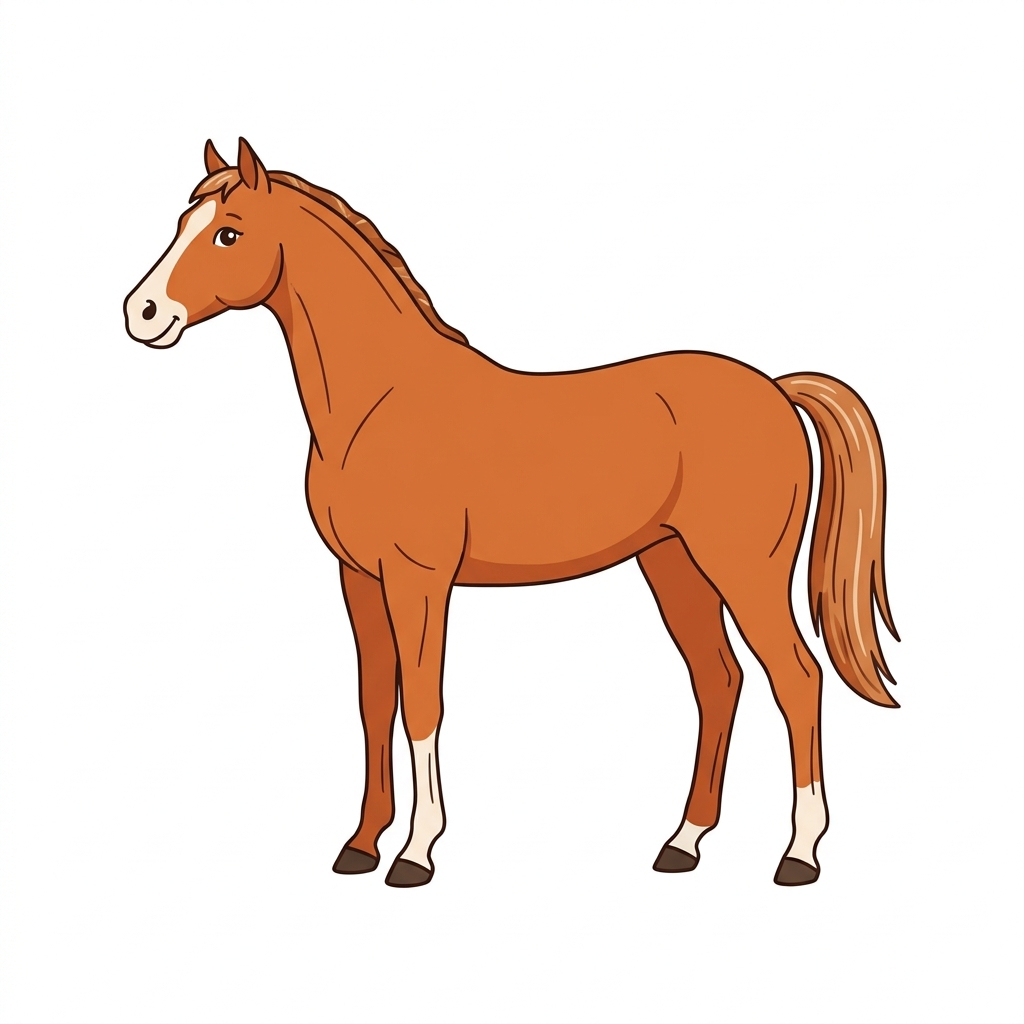
\includegraphics[width=0.9\linewidth]{vokab_300dpi/mier_femelle.png} \\
            \small\textit{Eng Mier (La jument / The mare)}
            \vspace{0.5cm}
        }}
    \end{minipage}
    
    \vspace{1.5em}
    
    \begin{minipage}[t]{0.48\textwidth}
        \centering
        \textbf{Eng Wëndel}
        \vspace{0.5em}
        \framebox{\parbox{0.9\linewidth}{\centering
            \vspace{0.5cm}
            
\includegraphics[width=0.9\linewidth]{vokab_300dpi/wendel.png} \\
            \small\textit{Eng Wëndel (La couche / The diaper)}
            \vspace{0.5cm}
        }}
    \end{minipage}
    \hfill
    \begin{minipage}[t]{0.48\textwidth}
        \centering
        \textbf{Eng Fatz}
        \vspace{0.5em}
        \framebox{\parbox{0.9\linewidth}{\centering
            \vspace{0.5cm}
            
\includegraphics[width=0.9\linewidth]{vokab_300dpi/fatz.png} \\
            \small\textit{Eng Fatz (Le chiffon / The rag)}
            \vspace{0.5cm}
        }}
    \end{minipage}
    
    \vspace{1.5em}
    
    \begin{minipage}[t]{0.48\textwidth}
        \centering
        \textbf{E Fatzert}
        \vspace{0.5em}
        \framebox{\parbox{0.9\linewidth}{\centering
            \vspace{0.5cm}
            
\includegraphics[width=0.9\linewidth]{vokab_300dpi/fatzert.png} \\
            \small\textit{E Fatzert (Le vaurien / The scoundrel)}
            \vspace{0.5cm}
        }}
    \end{minipage}
\end{center}
